As mentioned in \autoref{sec:design-and-system-architecture}, the software for the system is written in Python and is run entirely on the Raspberry Pi 4B. The software is divided into three main components: the user interface, the computer vision system, and the system controller which manages the hardware components of the system. The software is designed to be modular, with each component being able to run independently of the others. This allows for easier debugging and testing of the system, as well as making it easier to add new features in the future.

\subsubsection{User Interface}
The user interface allows the user to view and command the state of the system by interacting with the touchscreen on the DFRobot 7" display. From here, the user is able to\dots

\begin{figure}[H]
    \hfill
    \begin{minipage}[t]{\textwidth}
      \centering
      \includegraphics[width=\textwidth,height=5cm, keepaspectratio]{example-image-a}
      \caption{User Interface}
      \label{fig:ui}
    \end{minipage}
\end{figure}

As shown in \autoref{fig:ui}, the user interface consists\dots

Written in pygame \cite{pygamedoc} and pygame\_gui \cite{pygamegui}, the user interface is controlled by the \texttt{LCD\_UI} class, which is responsible for drawing the various elements of the user interface, such as the camera feed, the buttons, and the text. The system operates at 30Hz, allow for responsiveness without overloading the system. A profiler was used to determine the performance of the system, and it was found that the system was able to run at 30Hz without any issues as discussed in \autoref{sec:evaluation}.

The user interface also supports a "training mode", where the camera feed is enlarged in order to capture images of components to be used for training the computer vision system, done programmatically by toggling a flag called \texttt{TRAININGMODE} in the \texttt{LCD\_UI} class. This is only used during the dataset collection phase of the project, and is not used during the normal operation of the system. This is discussed in more detail in \autoref{sec:dataset-collection}.

\begin{figure}[H]
    \hfill
    \begin{minipage}[t]{\textwidth}
      \centering
      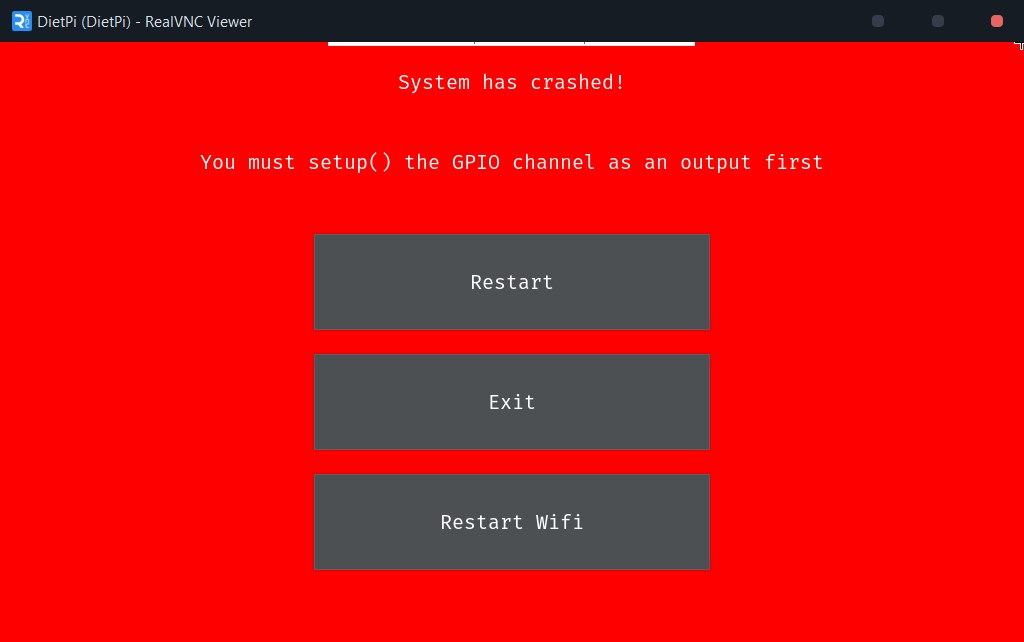
\includegraphics[width=\textwidth]{imgs/python/systemcrash.jpg}
      \caption{System crash during development}
      \label{fig:crash}
    \end{minipage}
\end{figure}

The LCD UI class is also capable of gracefully handling errors that may occur during the operation of the system, and the handling of these errors is delegated to the specific subsystem that caused the error. If a much more catastrophic error occurs, the system will still gracefully display an error screen, and allow the system to be restarted as shown in \autoref{fig:crash}. This facilitates not only the development process, but also prevents the system from having downtime in real-world applications as it prevents the need for a system restart. This is implemented by making use of Python's exception handling mechanism, and then switching to the error screen if an exception is raised.

The camera feed in the top left is controlled by the Vision Handler, which is responsible for delivering frames to the user interface. The Vision Handler is discussed in more detail in \autoref{sec:vision-handler}. 
\todo{Complete section after fully implementing the user interface}

\subsubsection{Vision Handler}
\label{sec:vision-handler}
The Vision Handler is responsible for managing the camera feed, and performs the following tasks:
\begin{mylist}
    \item Capturing frames from the camera
    \item Performing inference by passing the frames to the computer vision model
    \item Gracefully handling errors that may occur during inference
    \item Gracefully handling capture errors (such as the camera being disconnected)
    \item The ability to live capture from the \texttt{TRAININGMODE=True} UI mode to allow for development off the Raspberry Pi
\end{mylist}

\autoref{fig:camera-disconnect} shows what the user interface displays when the camera is disconnected.

\begin{figure}[H]
    \hfill
    \begin{minipage}[t]{\textwidth}
      \centering
      \includegraphics[width=\textwidth, height=10cm]{example-image-b}
      \caption{Camera disconnect error}
      \label{fig:camera-disconnect}
    \end{minipage}
\end{figure}

\subsubsection{Dataset Collection}
\label{sec:dataset-collection}
As mentioned in \autoref{sec:data-annotation-tool}, a custom dataset annotation tool was used to collect and annotate the dataset required to train the YOLO-OBB model used for component identification, and then extended to train a regular YOLO model for resistor value detection.

\begin{figure}[H]
    \hfill
    \begin{minipage}[t]{\textwidth}
      \centering
      \includegraphics[width=\textwidth, height=10cm]{example-image-c}
      \caption{Training mode screen}
      \label{fig:training-mode}
    \end{minipage}
\end{figure}

As shown in \autoref{fig:training-mode}, to facilitate the collection of the dataset, the user interface was modified to include a "training mode" that allows the user to capture images of components to be used for training the computer vision system. As the camera feed must originate from the Pi, dataset collection is done on a machine connected to the Pi with VNC \cite{realvnc}, and the user interface is displayed on the VNC client. When \texttt{TRAININGMODE} is enabled, a purple border surrounds the camera feed, enabling the dataset tool to identify where the camera feed is located on the VNC window.

The tool makes use of keybinds to capture images, to allow the user to capture images of components quickly, detailed in the following table:

\begin{table}[H]
    \centering
    \begin{tabularx}{0.8\textwidth}{|p{2cm}|X|}
        \hline
        \textbf{Key} & \textbf{Action} \\
        \hline
        \texttt{Space} & Capture from VNC window \\
        \hline
        \texttt{Enter} & Save image but only if the image is captured and labelled \\
        \hline
        \texttt{Escape} & Return to the component selection screen \\
        \hline
    \end{tabularx}
    \caption{Main keybinds for the dataset collection tool}
    \label{tab:keybinds}
\end{table}



